\documentclass[a4paper]{article}
\usepackage[utf8]{inputenc}
\usepackage[english]{babel}
\usepackage{csquotes}
\usepackage{amsmath} % per ambienti tipo cases
\usepackage{amssymb}
\usepackage{mathtools}
\usepackage{siunitx}
\usepackage{graphicx} % per includere figure
%\usepackage{subfigure}
\usepackage{booktabs} % per le tabelle
\usepackage{caption}
\usepackage{fancyhdr}
\usepackage{hyperref}
\usepackage[section]{placeins}
\usepackage{microtype}
\usepackage{caption}
\usepackage{subcaption}
\captionsetup[subfigure]{labelfont=rm}
\usepackage{verbatim} %multiline comments
\usepackage{wrapfig}
\usepackage[backend=biber, style=numeric, safeinputenc, sorting=none]{biblatex}
\addbibresource{source.bib}	% uncomment for bibliography



%opening
\title{}
\author{}

\pagestyle{fancy}
\lhead{Musical Acoustics}
\chead{H7}
\rhead{10743504, 10751919}
\newcommand{\Rarrow}{\mbox{\Large$\Rightarrow$}}

\begin{document}

\begin{titlepage}	
	\newcommand{\HRule}{\rule{\linewidth}{0.5mm}} % Defines a new command for horizontal lines, change thickness here
	
	\center % Centre everything on the page
	
	%------------------------------------------------
	%	Headings
	%------------------------------------------------
	
	
\includegraphics[width=.4\textwidth]{Logo_Politecnico_Milano.png}\\[0.4cm]
	\textsc{\LARGE}\\[0.3cm] % Main heading such as the name of your university/college
	
	\textsc{\large MSc. Music and Acoustic Engineering}\\[1cm] % Minor heading such as course title
	
	\textsc{\Large Musical Acoustics - A.Y. 2020/2021}\\[0.5cm] % Major heading such as course name
	
	%------------------------------------------------
	%	Title
	%------------------------------------------------
	
	\HRule\\[0.4cm]
	
	{\huge\bfseries H7 - Eigenfrequency Study of a Marimba Bar }\\[0.4cm] % Title of your document
	
	\HRule\\[1.5cm]
	
	
	
	{\large\textit{Authors' IDs:}}\\
	10743504, 10751919, % Your name
	%\\ \textsc{Gruppo 11}
	
	%------------------------------------------------
	%	Date
	%------------------------------------------------
	
	\vfill\vfill\vfill % Position the date 3/4 down the remaining page
	
	{\large\today} % Date, change the \today to a set date if you want to be precise
	
	%------------------------------------------------
	%	Logo
	%------------------------------------------------
	
	\vfill\vfill
	%\includegraphics[width=0.2\textwidth]{Politecnico_di_Milano.eps}\\[1cm] % Include a department/university logo - this will require the graphicx package
	
	%----------------------------------------------------------------------------------------
	
	\vfill % Push the date up 1/4 of the remaining page
	
	
\end{titlepage}

\section{Constructing the mesh}

\begin{figure}[h]
	\centering
	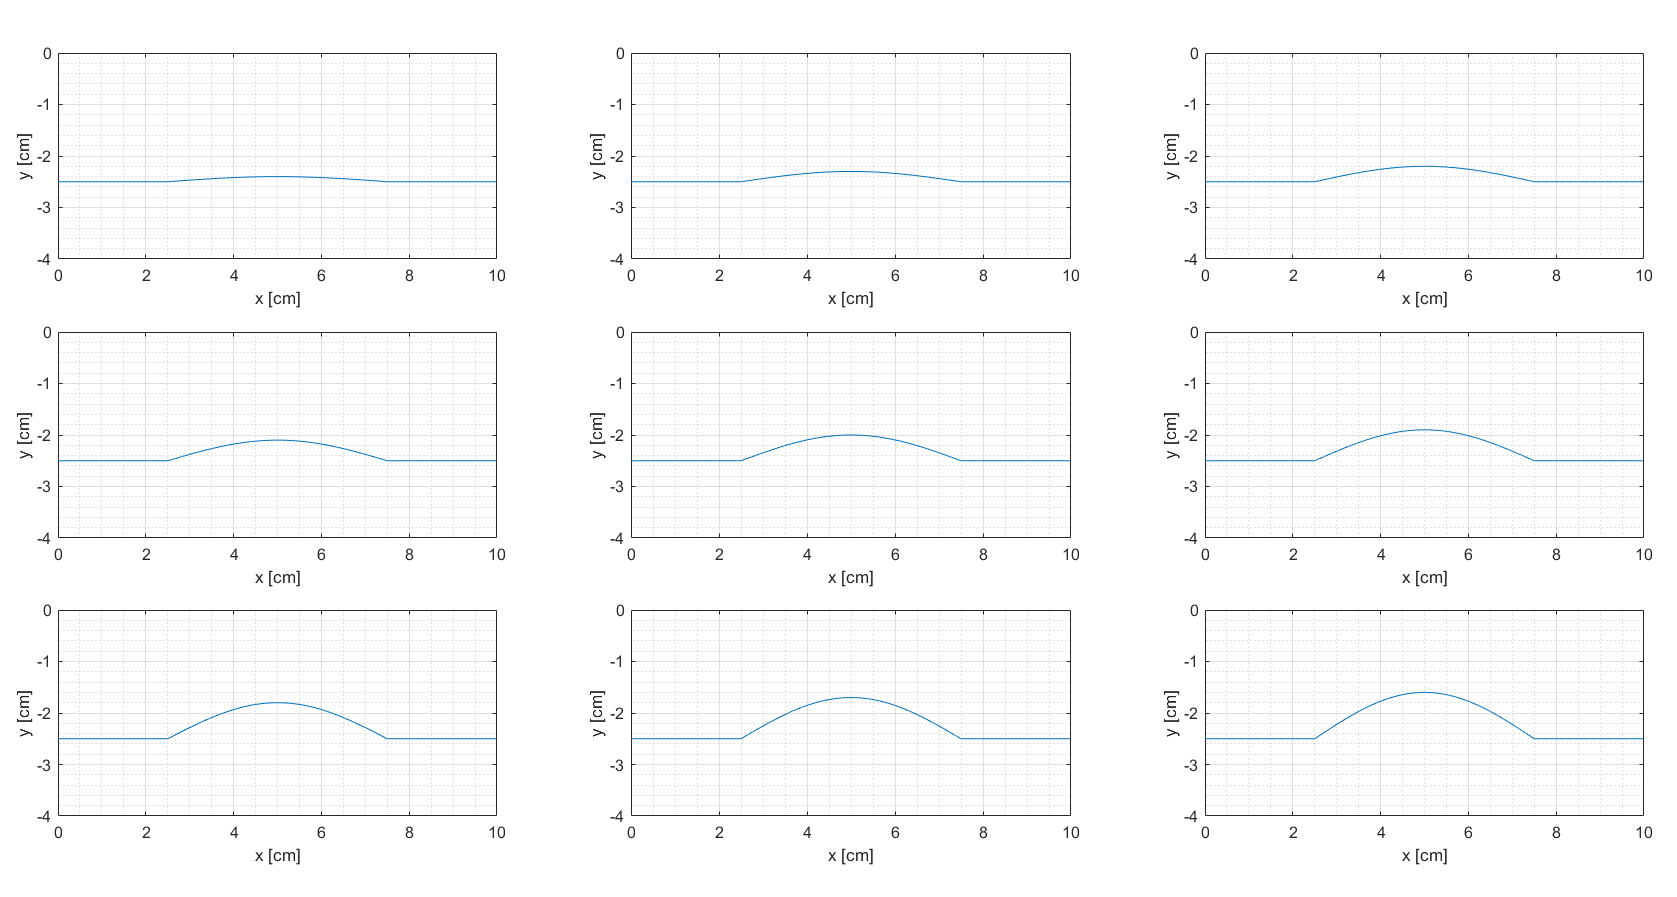
\includegraphics[width=0.7\linewidth]{barshapes.png}
	\caption{Profiles of the lower surface of a marimba bar with the depth of the arching varying from 1 to 9 mm.}
	\label{fig:profiles}
\end{figure}

Our aim in this homework is to study the dependency of the modes of a marimba bar on the depth $a$ of the arching. Fig. \ref{fig:profiles} shows how we modelled the profiles: the cutaway is sinusoidal in shape and varies from 1 to 9 mm in depth in steps of 1 mm. The model for the bar was implemented in Comsol with a length of 10 cm, a height of 2.5 cm and a width of 2.5 cm. The depth $a$ was defined as a global parameter in order to perform a parametric study of the eigenfrequencies. The values of the Young moduli, shear moduli and Poisson coefficients were taken from \cite{wood}, considering Honduran mahogany as our material of choice. Ideally, the most sought after instruments of this kind are made of rosewood; however, for this material, it is harder to find measurements of all of the nine relevant parameters that are needed to completely characterize it. Fig. \ref{fig:mesh} shows the profiles of the generated meshes.

\begin{figure}[h]
	\centering
	\begin{subfigure}{0.22\linewidth}
		\centering
		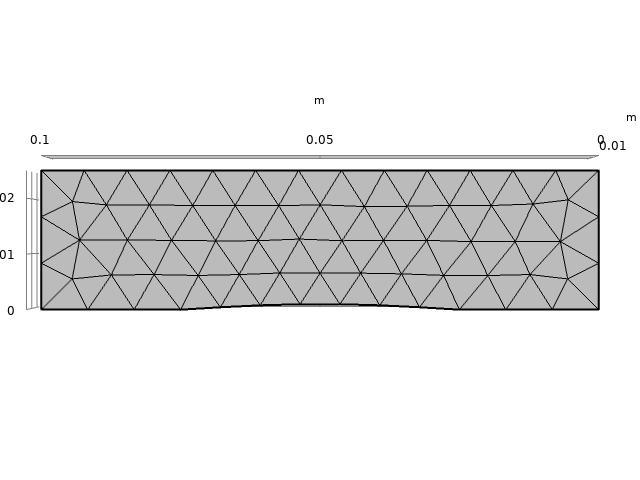
\includegraphics[width=0.95\linewidth]{01.jpg}
	\end{subfigure}
	~
	\begin{subfigure}{0.22\linewidth}
		\centering
		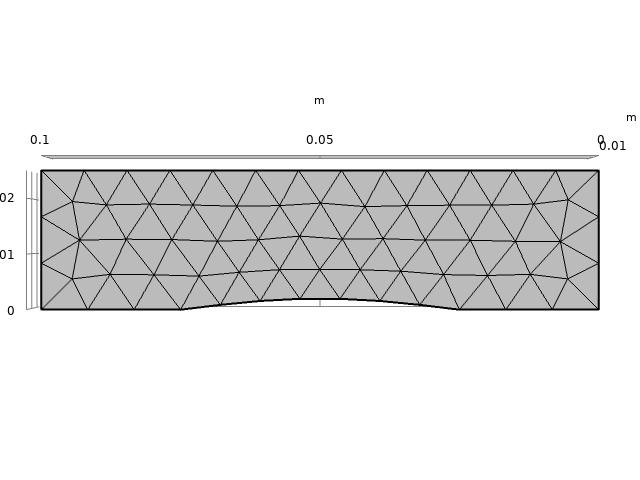
\includegraphics[width=0.95\linewidth]{02.jpg}
	\end{subfigure}
	~
	\begin{subfigure}{0.22\linewidth}
		\centering
		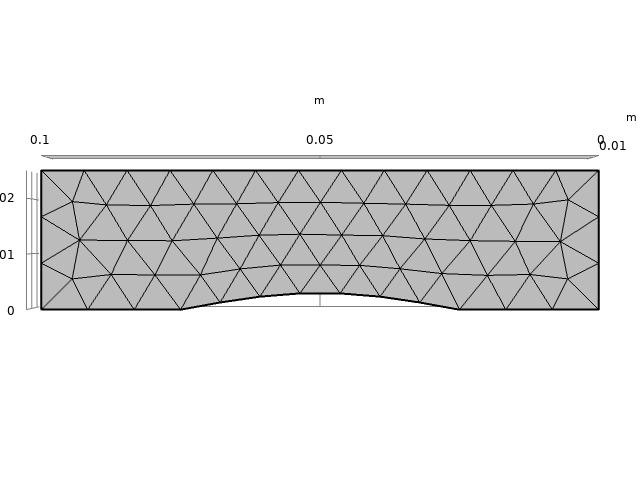
\includegraphics[width=0.95\linewidth]{03.jpg}
	\end{subfigure}

	\begin{subfigure}{0.22\linewidth}
		\centering
		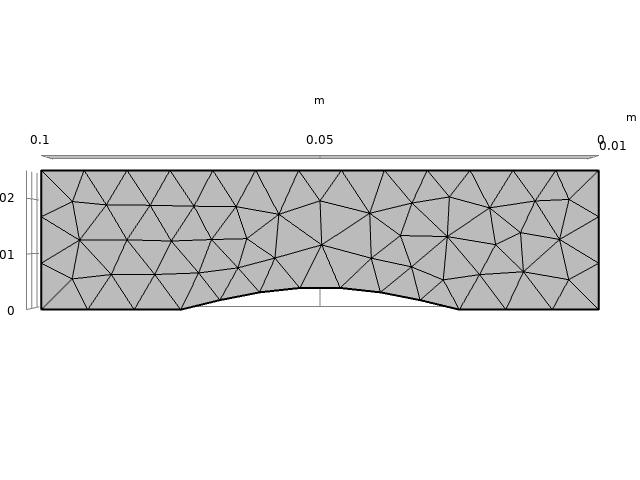
\includegraphics[width=0.95\linewidth]{04.jpg}
	\end{subfigure}
	~
	\begin{subfigure}{0.22\linewidth}
		\centering
		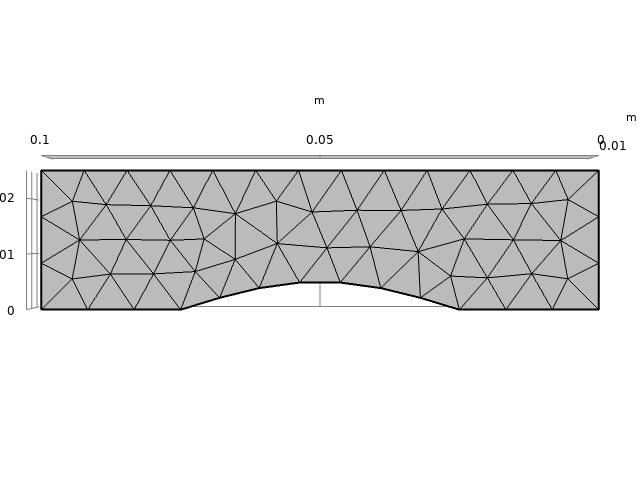
\includegraphics[width=0.95\linewidth]{05.jpg}
	\end{subfigure}
	~
	\begin{subfigure}{0.22\linewidth}
		\centering
		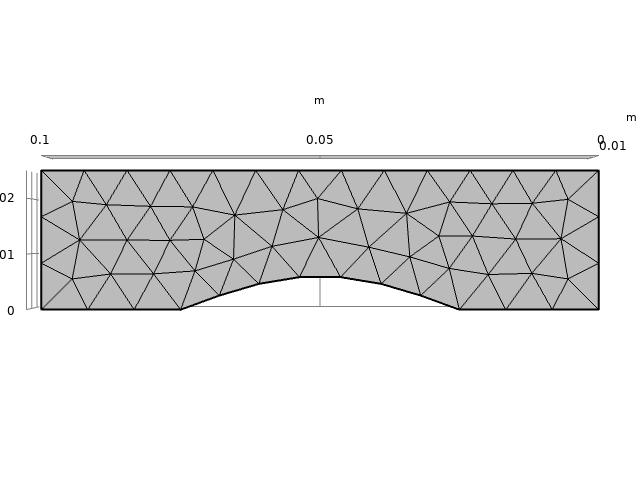
\includegraphics[width=0.95\linewidth]{06.jpg}
	\end{subfigure}

	\begin{subfigure}{0.22\linewidth}
		\centering
		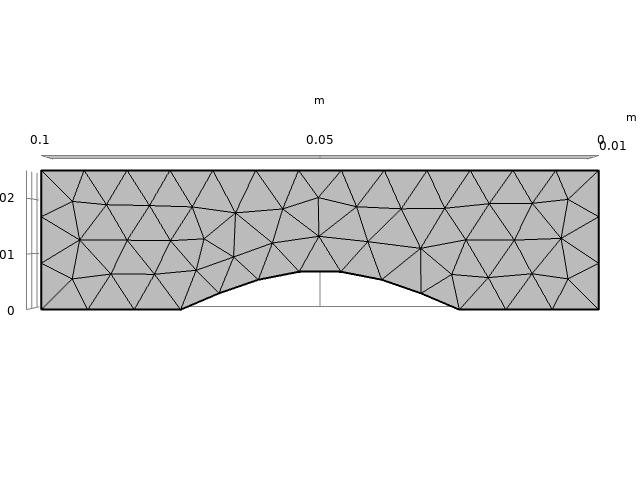
\includegraphics[width=0.95\linewidth]{07.jpg}
	\end{subfigure}
	~
	\begin{subfigure}{0.22\linewidth}
		\centering
		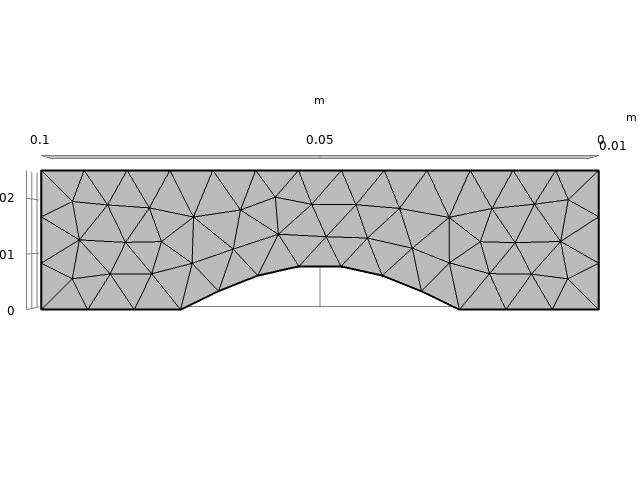
\includegraphics[width=0.95\linewidth]{08.jpg}
	\end{subfigure}
	~
	\begin{subfigure}{0.22\linewidth}
		\centering
		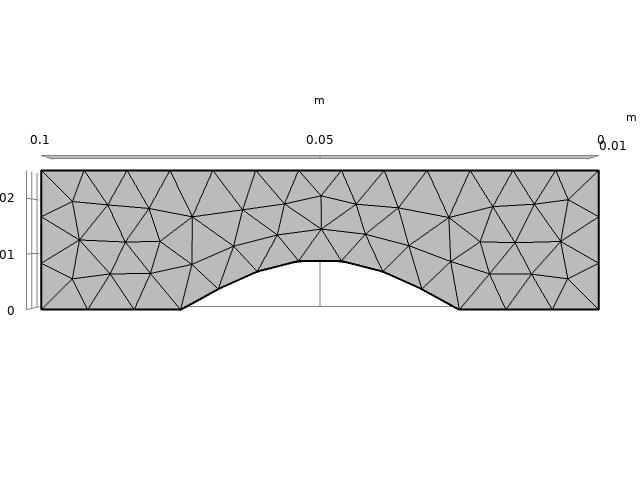
\includegraphics[width=0.95\linewidth]{09.jpg}
	\end{subfigure}
	\caption{Profiles of the Comsol mesh for all values of $a$ used in the parametric study.}
	\label{fig:mesh}
\end{figure}

\section{Eigenfrequencies}
As mentioned in the previous section, a parametric eigenfrequency study was performed, with the values we already reported for $a$ and with free boundary conditions. The first five eigenfrequencies obtained from this study for each value of $a$ are reported in Tab. \ref{tab:freqs}. They are also reported as functions of $a$ in Fig. \ref{fig:freqz}.

\begin{table}[h]
	\centering
	$\begin{array}{l|ccccccccc}
		\toprule
		 a~[\si{\centi\meter}] & 0.1 & 0.2 & 0.3 & 0.4 & 0.5 & 0.6 & 0.7 & 0.8 & 0.9\\
		 \midrule
		 f_1[\si{\kilo\hertz}]&5.9071  &  5.7717  &  5.6294  &  5.4788   & 5.3202 &   5.1534  &  4.9770  &  4.7969   & 4.6076\\
		 f_2[\si{\kilo\hertz}]&8.1063   & 8.0827 &   7.8760  &  7.5803  &  7.2655 &   6.9319  &  6.5852  &  6.2287 &   5.8557\\
		 f_3[\si{\kilo\hertz}]&8.4015  &  8.1523  &  8.0464  &  8.0000  &  7.9430 &   7.8755 &   7.7968  &  7.7086 &   7.6096\\
		 f_4[\si{\kilo\hertz}]&12.2164 &  12.3037 &  12.3886  & 12.4762 &  12.5592 &  12.6413 &  12.7214  & 12.7876 &   12.5428\\
		 f_5[\si{\kilo\hertz}]&14.0013  & 13.8828 &  13.7447  & 13.5885  & 13.4160&   13.2263 &  13.0134 &  12.7992 &  12.8797\\
		 \bottomrule
	\end{array}$
	\caption{First five eigenfrequencies of the bar for each value of $a$.}
	\label{tab:freqs}
\end{table}

\begin{figure}[h]
	\centering
	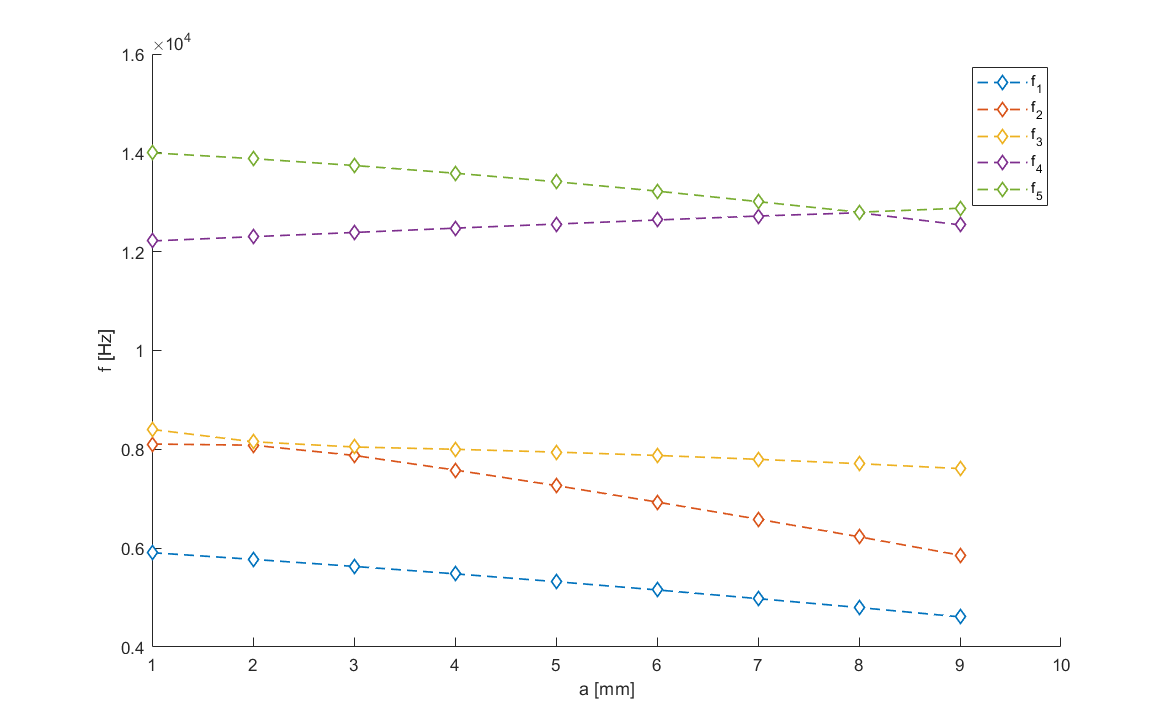
\includegraphics[width=0.85\linewidth]{freqz.png}
	\caption{The five lowest eigenfrequencies plotted as functions of $a$.}
	\label{fig:freqz}
\end{figure}


\section{Inharmonicity}

Lastly, we compute the inharmonicity of the sets of eigenfrequencies obtained before. The inharmonicity is a descriptor defined as:
\begin{gather*}
	I = \sum_{n=2}^{N} \left| \frac{f_n}{f_{n-1}} - m_n \right|, \\
	m_n = \arg \underset{m}{\min} \left| f_n - m f_{n-1} \right|,~ m \in \mathbb{N}^+,
\end{gather*}
where $N=5$ in our case. The values of $I$ we computed are reported in Fig. \ref{fig:inharm}.

\begin{figure}[h]
	\centering
	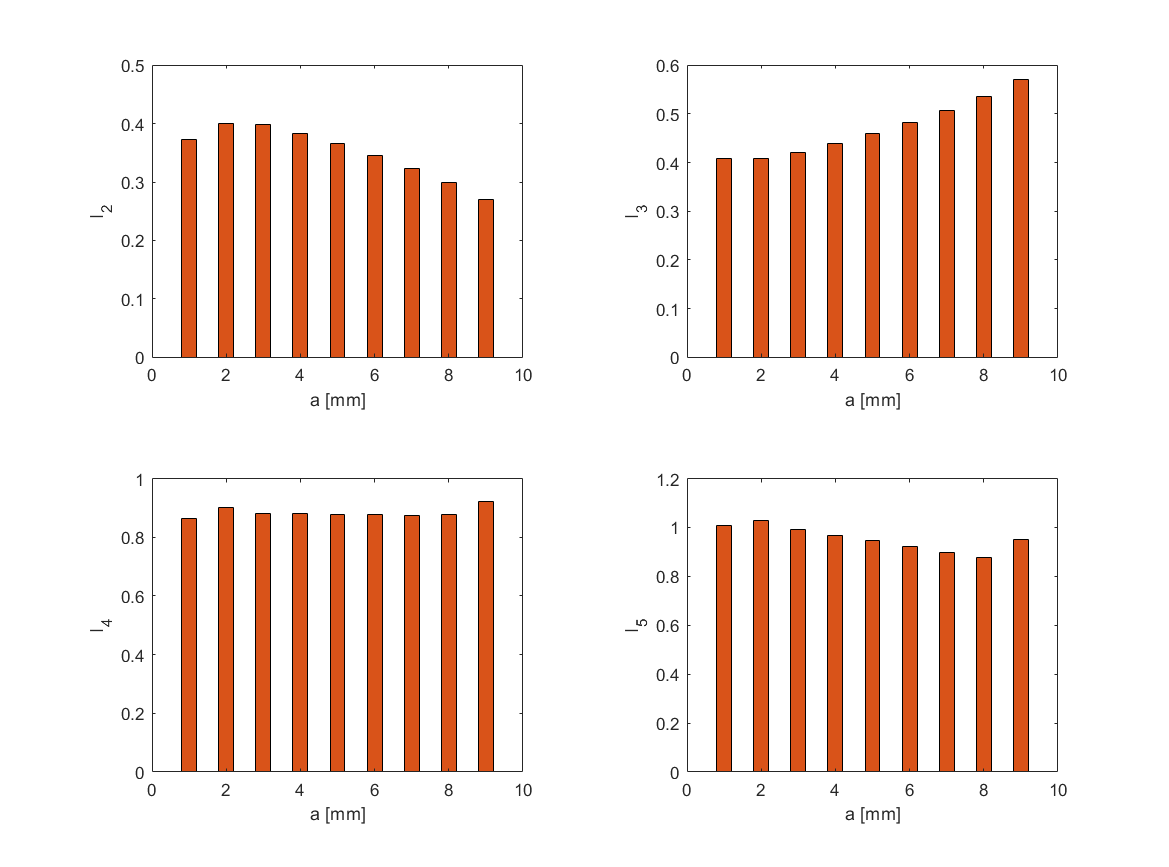
\includegraphics[width=0.85\linewidth]{inharmonicity.png}
	\caption{Inharmonicity as a function of $a$.}
	\label{fig:inharm}
\end{figure}

\section{A better shape of the bar}

Looking at the values we obtained from the eigenfrequency study, a problem seems to arise. While we expect the values of the ratios between the frequencies of the first two bending modes












\end{document} 